\documentclass[xcolor=pdftex,dvipsnames,table]{beamer}
\usepackage{beamerthemesplit}
\usetheme{Copenhagen}
\useoutertheme{shadow}
\useinnertheme{rounded}
\usepackage{color}
\usepackage{graphicx}
\usepackage{fancybox}


\title{Website Changes and User Behavior}
\subtitle{Using Panjiva Data to Examine Code Changes}
\author{John J. Wang}
\date{\today}
\institute{14.27 Final Presentation}

\begin{document}

\frame{\titlepage}

\frame{\tableofcontents}

\section[Introduction]{Introduction}

\frame{\tableofcontents[currentsubsection]}

\subsection{Silicon Valley Mindset}

\frame{
    \frametitle{The Silicon Valley Mindset}
    \begin{itemize}
        \item "Move fast and break things." -- Facebook
        \item "The only constant is change itself." -- Heraclitus
        \item "Pick a movement, pick a revolution, and join it." -- Jack Dorsey
    \end{itemize}
}

\subsection{What We Know}

\frame{\tableofcontents[currentsubsection]}

\frame
{
    \frametitle{Background and Previous Research}
    \begin{itemize}
        \item Academia has little to say on code changes and user behavior
        \item Most of the data is hidden away in large tech companies
        \item Although these companies probably run experiments, results aren't necessarily made public
    \end{itemize}
}

\subsection{Questions to Ask}

\frame{\tableofcontents[currentsubsection]}

\frame
{
    \frametitle{Lingering Questions}
    \begin{itemize}
        \item Do users tend to respond favorably to website changes?
        \item How do users react to different types of change?
        \item How do different characteristics of users affect their reactions to change?
    \end{itemize}
}

\subsection{Panjiva Dataset}

\frame{\tableofcontents[currentsubsection]}

\frame
{
    \frametitle{Panjiva, Inc.}
    \begin{itemize}
        \item \url{http://www.panjiva.com}
        \item Acts as a medium for buyers and suppliers of manufactured goods
        \item Example: Home Depot finding a wrench factory
    \end{itemize}
}

\frame
{
    \frametitle{Commit Statistics}
    \begin{table}[h!]
    \centering
    \caption{Overall Commit Statistics - 11/25/2012}
    \begin{tabular}{l || l }
    \hline
    Active Days (at least 1 commit) & 1,983 \\
    Total Current Files & 20,901 \\
    Total Lines of Code & 1,313,235 \\
    Total Lines of Code Added & 3,989,295 \\
    Total Lines of Code Removed & 2,676,060 \\
    Total Commits & 29,924 \\
    Total Authors/Developers & 33 \\
    \hline
    \end{tabular}
    \label{table:commit-stats}
    \end{table}
} 

\section{Macro-Level Results}

\subsection{Daily Effects of Code Changes}

\frame{\tableofcontents[currentsubsection]}

\frame
{
    \frametitle{Specification}
    \begin{eqnarray}
    y^i_{t} = c_0 + \vec{\gamma}^T \vec{M}_t + \vec{\beta}^T \vec{\chi}_t + \epsilon_t
    \end{eqnarray}

    \begin{itemize}
        \item $t$ indexes day
        \item $y^i_t$ corresponds to $i$th metric of user activity on day $t$
        \item $\vec{M}_t$ corresponds to a vector of covariates that represent changes in the code
        \item $\vec{\chi}_t$ is a vector of controls
    \end{itemize}
}   

\frame
{
    \frametitle{Effect of Commits on User Activity}
    \begin{table}
    \scriptsize
    \centering
    {
        \def\sym#1{\ifmmode^{#1}\else\(^{#1}\)\fi}
        \begin{tabular}{l*{2}{c}}
        \hline\hline
            &\multicolumn{1}{c}{(1)}&\multicolumn{1}{c}{(2)}\\
            &\multicolumn{1}{c}{activitylogcount}&\multicolumn{1}{c}{eventlogcount}\\
            \hline
            fileschanged&     -5530.7         &    -60589.4\sym{*}  \\
 percentile           &     (-1.91)         &     (-2.26)   \\
            [1em]
            insertions&      4868.8\sym{*}  &     47053.7\sym{*} \\
percentile
    &      (2.12)         &      (2.22)         \\
        [1em]
        deletions&      2778.9         &     29970.6    \\
        percentile&      (1.29)         &      (1.50)   \\
        [1em]
        weekend     &    -14708.0\sym{***}&    -79769.8\sym{***}\\
        &    (-16.48)         &     (-9.65)      \\
        [1em]
        \_cons      &     22396.6\sym{***}&    224482.8\sym{***}\\
        &     (25.05)         &     (27.12)      \\
        \hline
        \(N\)       &         474         &         475     \\
        \hline\hline
        \multicolumn{3}{l}{\textit{t} statistics in parentheses}\\
        \multicolumn{3}{l}{\sym{*} \(p<0.05\), \sym{**} \(p<0.01\), \sym{***} \(p<0.001\)}\\
        \end{tabular}
    }
    \end{table}
}

\frame
{
    \frametitle{Effect of Commits on User Activity}
    \begin{table}[h!]
    \scriptsize
    \centering
    {
        \def\sym#1{\ifmmode^{#1}\else\(^{#1}\)\fi}
        \begin{tabular}{l*{2}{c}}
        \hline\hline
            &\multicolumn{1}{c}{(1)}&\multicolumn{1}{c}{(2)}\\
            &\multicolumn{1}{c}{avguseractivity}&\multicolumn{1}{c}{avguserevents}\\
            \hline
            fileschanged&     -10.40\sym{*}         &    -148.6  \\
 percentile           &     (-2.01)         &     (-1.52)   \\
            [1em]
            insertions&      2.817  &     79.92 \\
percentile
    &      (0.69)         &      (1.03)         \\
        [1em]
        deletions&      4.670        &    49.47    \\
        percentile&      (1.21)         &      (0.68)   \\
        [1em]
        weekend     &    -0.297&    257.0\sym{***}\\
        &    (-0.19)         &     (8.49)      \\
        [1em]
        \_cons      &     25.00\sym{***}&    340.6\sym{***}\\
        &     (15.58)         &     (11.24)      \\
        \hline
        \(N\)       &         474         &         475     \\
        \hline\hline
        \multicolumn{3}{l}{\textit{t} statistics in parentheses}\\
        \multicolumn{3}{l}{\sym{*} \(p<0.05\), \sym{**} \(p<0.01\), \sym{***} \(p<0.001\)}\\
        \end{tabular}
    }
    \end{table}
}

\subsection{Lagged Effects of Code Changes}

\frame{\tableofcontents[currentsubsection]}

\frame
{
    \frametitle{Specification}
    \begin{eqnarray}
    y^i_{tx} = c_0 + \gamma M_{t} + \beta weekend_{t} + \epsilon_t
    \end{eqnarray}

    \begin{itemize}
        \item Lag variable $x \in [1,30]$. 
        \item Examines how commits on day $t$ affect user behavior in time $t + x$. 
    \end{itemize}

}

\frame
{
    \frametitle{Average Activity Logs Per Distinct User}
    \begin{figure}[h!]
    \centering
    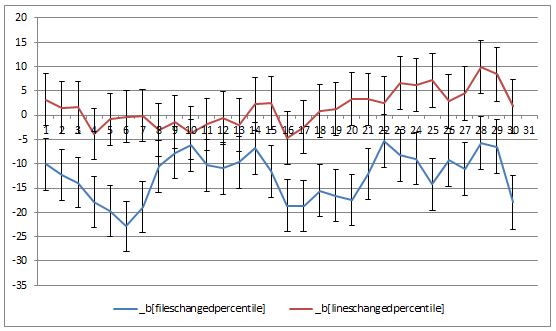
\includegraphics[width=3.8in]{pictures/avg_activities_time_coefficients.png}
    \label{fig:avg-activities-time-coefficients}
    \caption{$\gamma$ Coefficients with Varying Lags, Regressed on Average Activity Logs per User}
    \end{figure}
}

\section{Micro-Level Results}

\subsection{Why Micro-Level Data?}

\frame{\tableofcontents[currentsubsection]}

\frame
{
    \frametitle{Problems with Macro-Level Data}
    \begin{itemize}
    \item Nothing more than correlations
    \item Possibly complex, unknown mechanisms for how results come about
    \end{itemize}
}

\frame
{
    \frametitle{The Case for Micro-Level Data}
    \begin{itemize}
    \item Panjiva has data on the page and time that any action was performed.
    \item Code changes (commits) can be thought of as exogeneous shocks.
    \item Almost all changes are unannounced
    \item Only extremely large changes are announced on blog (less than 1\% of Panjiva's total pageviews come from blog).
    \end{itemize}
}

\subsection{Search Controller}

\frame{\tableofcontents[currentsubsection]}

\frame
{
    \frametitle{Search Controller}
    \begin{figure}
    \centering
    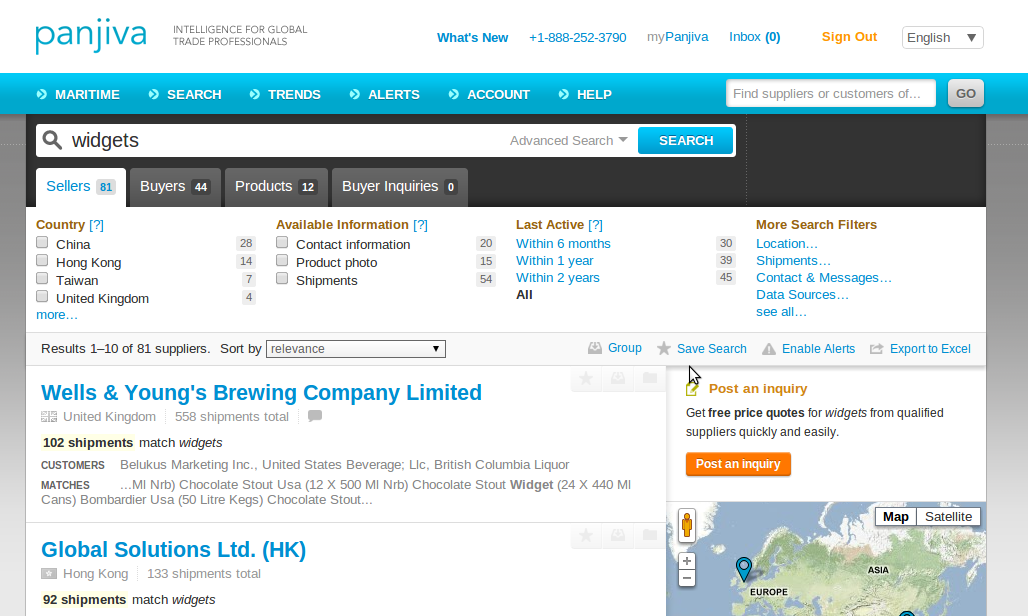
\includegraphics[width=3in]{pictures/search_page.png}
    \caption{The Search Page, Panjiva's most trafficked page, provides functionality for finding suppliers, buyers, products, and buyer inquiries.}
    \end{figure}
}

\frame
{
    \frametitle{Visualization of Variables}
    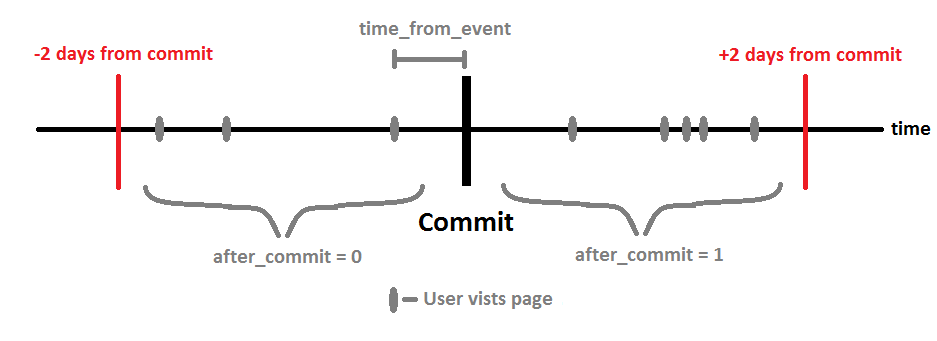
\includegraphics[width=4.5in]{pictures/specification_diagram.png}

}

\frame
{
    \frametitle{Search Regression Results}
    \begin{table}
    \scriptsize
    \centering
    {
        \def\sym#1{\ifmmode^{#1}\else\(^{#1}\)\fi}
        \begin{tabular}{l*{4}{c}}
        \hline\hline
            & \multicolumn{4}{l}{Dependent Variable: num\_views\_day\_later} \\
            &\multicolumn{1}{c}{(1)}&\multicolumn{1}{c}{(2)}&\multicolumn{1}{c}{(3)}&\multicolumn{1}{c}{(4)}\\
            \hline
            after\_commit&       5.541\sym{***}&               &       3.378\sym{***}&                     \\
            &     (17.91)         &                     &     (11.20)         &                     \\
            [1em]
            time\_from\_event&                     &   0.0000737\sym{***}&                     &    0.000110\sym{***}\\
            &                    &     (43.76)         &                     &     (66.60)         \\
            [1em]
            created\_at\_hour&             No        &           No           &       Yes &      Yes \\
            dummies?&                     &                     &              &            \\
            [1em]
            \_cons      &       156.9\sym{***}&       159.9\sym{***}&       138.3\sym{***}&       139.7\sym{***}\\
            &    (731.32)     &   (1033.47)         &    (127.71)         &    (130.50)         \\
            \hline
            \(N\)       &     2345617       &     2345617         &     2345617         &     2345617         \\
            \hline\hline
            \multicolumn{5}{l}{\scriptsize \textit{t} statistics in parentheses, \sym{*} \(p<0.05\), \sym{**} \(p<0.01\), \sym{***} \(p<0.001\)}\\
            \end{tabular}
    }
    \end{table}
}

\subsection{Commit Types}

\frame{\tableofcontents[currentsubsection]}

\frame
{
    \frametitle{Specification}
    \begin{eqnarray}
    num\_views\_day\_later_{it} &=& \beta_0 after\_commit_{it} + \beta_1 insertionspercentile_{it} + \beta_2 deletionspercentile_{it} \\ \nonumber
    &+& \beta_3 insertionspercentile_{it} * after\_commit_{it} \\ \nonumber
    &+& \beta_4 deletionspercentile_{it} * after\_commit_{it} \\ \nonumber
    &+& \beta_5 hour\_dummies_{it} + c_0 +  \epsilon_{it}
    \end{eqnarray}

    \begin{itemize}
        \item Interaction term coefficients $\beta_3$ and $\beta_4$ give incremental percentile coefficients after the commit
        \item Same specification, but including interaction terms to see additive effect
    \end{itemize}
}

\frame
{
    \frametitle{Differences in Commits}
    \begin{table}
    \centering
    \scriptsize
    {
        \def\sym#1{\ifmmode^{#1}\else\(^{#1}\)\fi}
        \begin{tabular}{l*{4}{c}}
        \hline\hline
            & \multicolumn{4}{c}{Dependent Variable: num\_views\_day\_later} \\
            &\multicolumn{1}{c}{(1)}&\multicolumn{1}{c}{(2)}&\multicolumn{1}{c}{(3)}&\multicolumn{1}{c}{(4)}\\
            \hline
            after\_commit&      -10.86\sym{***}&      -13.79\sym{***}&      -325.5\sym{***}&      -305.9\sym{***}\\
            &    (-16.90)         &    (-22.03)         &   (-154.63)         &   (-149.28)         \\
            [0.5em]
            insertionspercentile&      -50.97\sym{***}&      -50.76\sym{***}&      -650.6\sym{***}&      -609.5\sym{***}\\
            &    (-54.12)         &    (-55.34)         &   (-218.09)         &   (-209.88)         \\
            [0.5em]
            deletionspercentile&       66.31\sym{***}&       63.35\sym{***}&       251.5\sym{***}&       230.8\sym{***}\\
            &     (70.67)         &     (69.34)         &     (84.73)         &     (79.94)         \\
            [0.5em]
            insertionspercentile *&       57.00\sym{***}&       58.05\sym{***}&       393.0\sym{***}&       365.1\sym{***}\\
            after\_commit&     (41.21)         &     (43.09)         &     (89.07)         &     (85.01)         \\
            [0.5em]
            deletionspercentile * &      -24.16\sym{***}&      -23.64\sym{***}&       2.306         &       3.295         \\
            after\_commit&    (-17.65)         &    (-17.74)         &      (0.53)         &      (0.77)         \\
            [0.5em]
            Hour Dummies?&      No               &    Yes &          No           &     Yes\\
            [0.5em]
            Controllers Used&      Search               &    Search &         All           &     All\\
            [0.5em]
            \_cons      &       150.1\sym{***}&       133.2\sym{***}&       606.5\sym{***}&       491.0\sym{***}\\
            &    (336.67)         &    (116.37)         &    (420.98)         &    (130.17)         \\
            \hline
            \(N\)       &     2345617         &     2345617         &     3858943         &     3858943         \\
            \hline\hline
        \end{tabular}
        }
    \end{table}
}

\subsection{Differential Controller Effects}

\frame{\tableofcontents[currentsubsection]}

\frame{
    \frametitle{Effects of Each Controller}
    \begin{eqnarray*}
    num\_views\_day\_later_{it} &=& \beta_0 after\_commit_{it} + \bar{\beta}_1 \overline{controllers}_{it} \\ \nonumber
    &+& \bar{\beta}_2 \overline{controllers}_{it}^T \times \overline{after\_commit}_{it} \\ \nonumber
    &+& \beta_3 hour\_dummies_{it} + \epsilon_{it} \nonumber
    \end{eqnarray*}

    \begin{itemize}
        \item Looking for the impact of controller $k$ on user activity after a commit
        \item Want to examine $\Gamma_k = \beta_{2k} + \beta_{1k} + \beta_0 - \beta_{1k} = \beta_{2k} + \beta_0$.
        \item Standard errors given by:
        \begin{eqnarray*}
        SE_{sum} = \sqrt{ SE_{cont_{2k}}^2 + SE_{ac}^2 + 2 Cov(cont_{2k}, ac)}
        \end{eqnarray*}

    \end{itemize}
}

\frame{
    \frametitle{Controller Results}
    \begin{table}
    \scriptsize
    \centering
    {
        \def\sym#1{\ifmmode^{#1}\else\(^{#1}\)\fi}
        \begin{tabular}{l*{2}{c}}
        \hline\hline
            &\multicolumn{1}{c}{(1)}&\multicolumn{1}{c}{(2)}\\
            &\multicolumn{1}{c}{No Hour Controls}&\multicolumn{1}{c}{With Hour Controls}\\
            \hline
            Communication & -2.673 & 5.111 \\
            & (-0.50) & (0.98) \\
            [.3em]
            My\_Panjiva & -41.718\sym{*} & -54.530\sym{***} \\
            & (-1.98) & (-2.68) \\
            [.3em]
            Profile & -8.167 & -6.339 \\
            & (-1.30) & (-1.04) \\
            [.3em]
            Project & -410.438\sym{***} & -388.496\sym{***} \\
            & (-235.55) & (-228.27) \\
            [.3em]
            Search & 5.541\sym{***} & 1.516 \\
            & (4.37) & (1.23) \\
            [.3em]
            US\_Exports & 10.318 & -28.946 \\
            & (0.28) & (-0.80) \\
            [.3em]
            US\_Imports & -12.487 & -8.73 \\
            & (-0.82) & (-0.59)\\
            \hline
            \(N\)       & 3858943  & 3858943   \\
            \hline \hline
        \end{tabular}
    }
    \end{table}
}

\section{Conclusion}

\frame{\tableofcontents[currentsection]}

\frame
{
    \frametitle{Conclusions}
    \begin{itemize}
        \item Code changes require particular factors for success
        \item Users respond negatively to low quality code (total and average user activity decreased when more files were changed)
        \item Changes to highly trafficked pages have greater chance of success
        \item Code changes can negatively affect user behavior
    \end{itemize}
}

\frame
{
    \frametitle{Acknowledgements}
    I would like to thank:
    \begin{itemize}
        \item Jim Psota
        \item Professor Ellison
        \item Panjiva, Inc.
    \end{itemize}
}

\end{document}


